\subsubsection{\large{Сервис запуска математических методов}}
\addcontentsline{toc}{subsubsection}

\begin{figure}[H]
	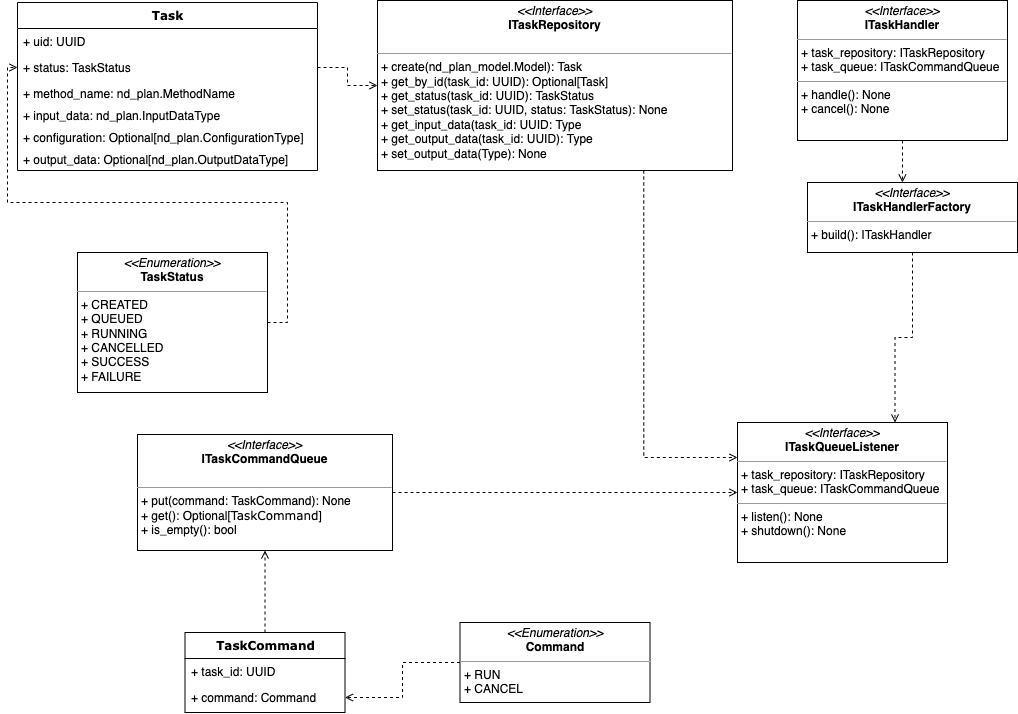
\includegraphics[width=\textwidth]{architecture/pictures/executor/execution_classes_diagram}
	\caption{Диаграмма классов расчетного модуля}
	\label{pic:architecture__execution-classes-diagram}
\end{figure}
\vskip 5 mm

Архитектура расчетного модуля представлена на диаграмме классов(см. рис\ \ref{pic:architecture__execution-classes-diagram}).
Основные классы и интерфейсы:
\begin{enumerate}
	\item \textit{Task} -- расчетная задача.
	\item \textit{TaskStatus} -- статус выполнения расчетной задачи.
	\item \textit{ITaskRepository} -- получения данных по расчётной задаче.
	\item \textit{ITaskHandler} -- запуск расчетных задач в отдельном процессе.
	\item \textit{ITaskCommandQueue} -- очередь задач.
	\item \textit{ITaskQueueListener} -- обработчик очереди задач, инициализация процесса расчета задач.
\end{enumerate}


\begin{figure}[H]
	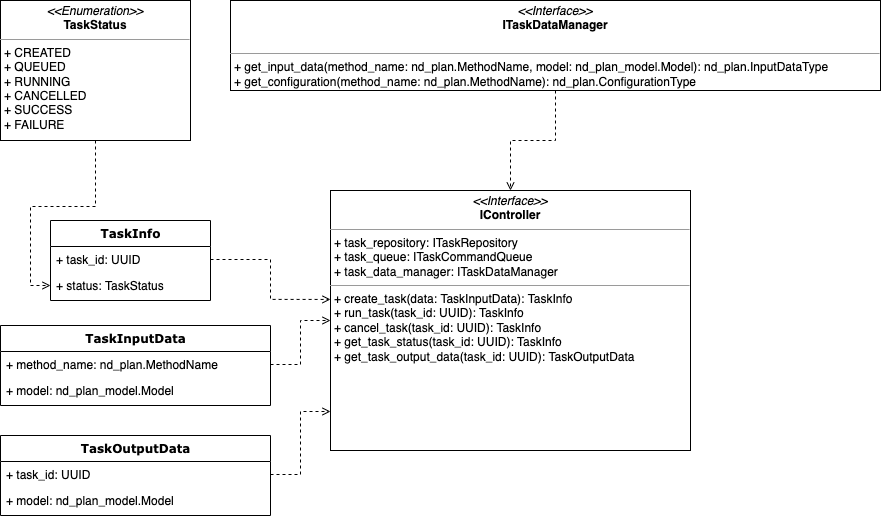
\includegraphics[width=\textwidth]{architecture/pictures/executor/api_classes_diagram}
	\caption{Диаграмма классов API}
	\label{pic:architecture__api-classes-diagram}
\end{figure}
\vskip 5 mm

Архитектура API представлена на диаграмме классов(см. рис\ \ref{pic:architecture__api-classes-diagram}).
Основные классы и интерфейсы:
\begin{enumerate}
	\item \textit{TaskInfo} -- информация о расчетной задаче.
	\item \textit{TaskStatus} -- статус выполнения расчетной задачи.
	\item \textit{TaskInputData} -- входные данные для создания расчетной задачи.
	\item \textit{TaskOutputData} -- результат расчета.
	\item \textit{ITaskDataManager} -- преобразование расчётной модели данных в модель данных математической библиотеки.
	\item \textit{IController} -- логика обработки запросов REST API.
\end{enumerate}